\section{Auswertung der Effizienz des Dashboards im Vergleich zum alten System}
% Usability = 
% - Efficiency: How quickly and with how much effort can users achieve their goals? This includes factors like time taken, number of steps, and cognitive load.
% Einfluss von Erlernbarkeit, Selbstbeschreibungsfähigkeit, Aufgabenangemessenheit
- Usability-Test -> Effizienz des Dashboards im Vergleich zum Legacy-System\\
-> Bewertung der Effizienz des Dashboards durch Gegenüberstellung der Testergebnisse\\

\begin{figure}[H]
    \centering
    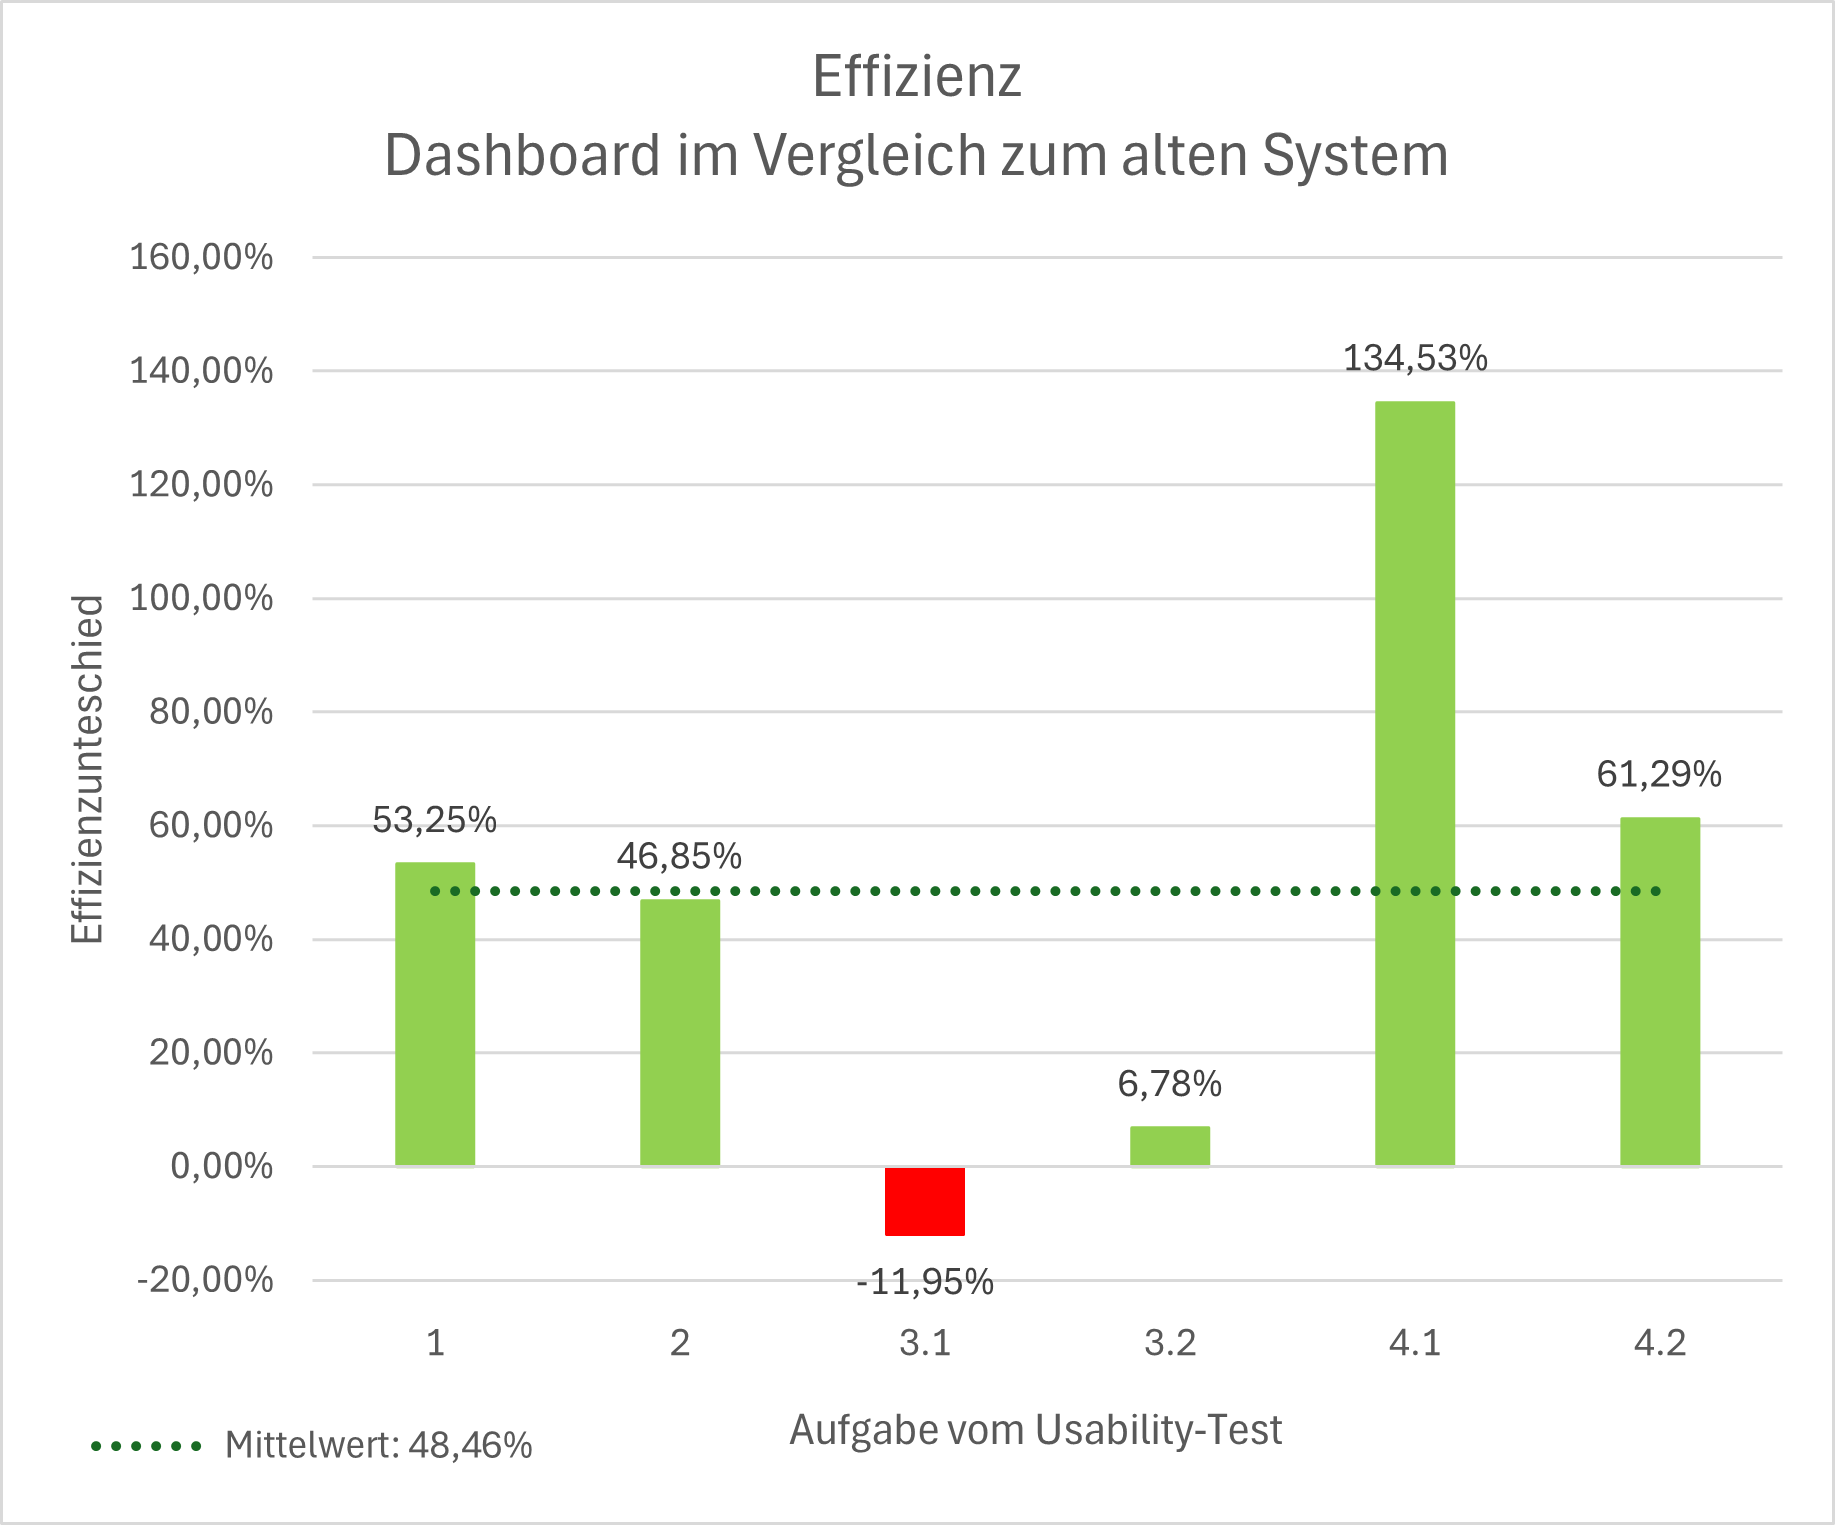
\includegraphics[width=0.8\linewidth]{Diagramme/usability_effizienz.png}
    \caption{Usability-Test: Effizienzvergleich vom neuen mit dem alten System\newline
    (Weiterverarbeitung der Daten aus \autoref{fig:usability_genauigkeit-zeit_alt-neu})}
    \label{fig:usability_effizienz}
\end{figure}

\subsection*{ISO-Kriterium Erlernbarkeit}
\begin{figure}[H]
    \centering
    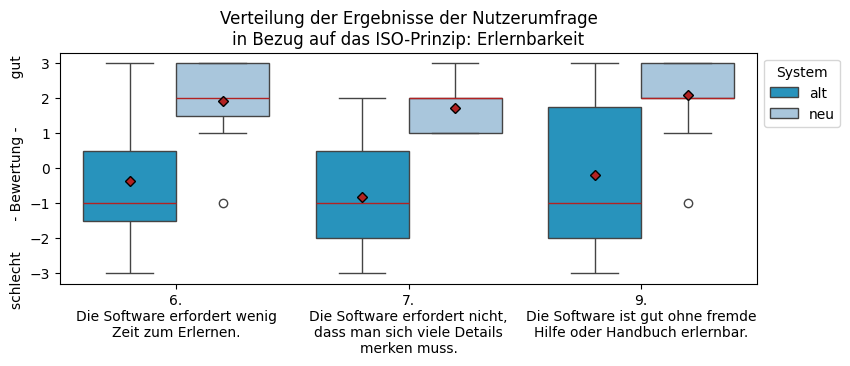
\includegraphics[width=1\linewidth]{Diagramme/pruemper_if.png}
    \caption{Auswertung der Fragen bzgl. Gestaltungskriterium Erlernbarkeit nach ISO 9241-110 (Ausschnitt aus \autoref{fig:pruemper_all})}
    \label{fig:pruemper_Erlernbarkeit}
\end{figure}

\noindent
t-Test von Fragen 6, 7 \& 9 sind signifikant (<0.5) - s. \autoref{tab:Nutzerbefragung:Differenz+ttest}\\
Boxplot: \autoref{fig:pruemper_Erlernbarkeit}
\subsection{ISO-Kriterium Selbstbeschreibungsfähigkeit}
\begin{figure}[H]
    \centering
    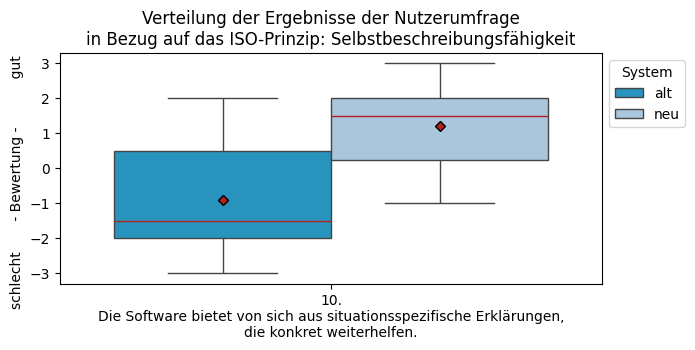
\includegraphics[width=1\linewidth]{Diagramme/pruemper_sb.png}
    \caption{Auswertung der Fragen bzgl. Gestaltungskriterium Selbstbeschreibungsfähigkeit nach ISO 9241-110 (Ausschnitt aus \autoref{fig:pruemper_all})}
    \label{fig:pruemper_Selbstbeschreibungsfähigkeit}
\end{figure}

\noindent
t-Test von Fragen 1 \& 8 sind signifikant (<0.5)\\
Boxplot: \autoref{fig:pruemper_Selbstbeschreibungsfähigkeit}

\subsection{ISO-Kriterium Aufgabenangemessenheit}
\autoref{fig:pruemper_Aufgabenangemessenheit}
\subsection{weitere: Steuerbarkeit, Erwartungskonformität, Robustheit gegen Benutzungsfehler}
